% Options for packages loaded elsewhere
\PassOptionsToPackage{unicode}{hyperref}
\PassOptionsToPackage{hyphens}{url}
%
\documentclass[
]{book}
\usepackage{amsmath,amssymb}
\usepackage{lmodern}
\usepackage{ifxetex,ifluatex}
\ifnum 0\ifxetex 1\fi\ifluatex 1\fi=0 % if pdftex
  \usepackage[T1]{fontenc}
  \usepackage[utf8]{inputenc}
  \usepackage{textcomp} % provide euro and other symbols
\else % if luatex or xetex
  \usepackage{unicode-math}
  \defaultfontfeatures{Scale=MatchLowercase}
  \defaultfontfeatures[\rmfamily]{Ligatures=TeX,Scale=1}
\fi
% Use upquote if available, for straight quotes in verbatim environments
\IfFileExists{upquote.sty}{\usepackage{upquote}}{}
\IfFileExists{microtype.sty}{% use microtype if available
  \usepackage[]{microtype}
  \UseMicrotypeSet[protrusion]{basicmath} % disable protrusion for tt fonts
}{}
\makeatletter
\@ifundefined{KOMAClassName}{% if non-KOMA class
  \IfFileExists{parskip.sty}{%
    \usepackage{parskip}
  }{% else
    \setlength{\parindent}{0pt}
    \setlength{\parskip}{6pt plus 2pt minus 1pt}}
}{% if KOMA class
  \KOMAoptions{parskip=half}}
\makeatother
\usepackage{xcolor}
\IfFileExists{xurl.sty}{\usepackage{xurl}}{} % add URL line breaks if available
\IfFileExists{bookmark.sty}{\usepackage{bookmark}}{\usepackage{hyperref}}
\hypersetup{
  pdfauthor={Leonardo F. Nascimento; Eric Brasil; Gabriel Andrade; Tarssio Barreto; Vítor Mussa; Daniel Mendes},
  hidelinks,
  pdfcreator={LaTeX via pandoc}}
\urlstyle{same} % disable monospaced font for URLs
\usepackage{longtable,booktabs,array}
\usepackage{calc} % for calculating minipage widths
% Correct order of tables after \paragraph or \subparagraph
\usepackage{etoolbox}
\makeatletter
\patchcmd\longtable{\par}{\if@noskipsec\mbox{}\fi\par}{}{}
\makeatother
% Allow footnotes in longtable head/foot
\IfFileExists{footnotehyper.sty}{\usepackage{footnotehyper}}{\usepackage{footnote}}
\makesavenoteenv{longtable}
\usepackage{graphicx}
\makeatletter
\def\maxwidth{\ifdim\Gin@nat@width>\linewidth\linewidth\else\Gin@nat@width\fi}
\def\maxheight{\ifdim\Gin@nat@height>\textheight\textheight\else\Gin@nat@height\fi}
\makeatother
% Scale images if necessary, so that they will not overflow the page
% margins by default, and it is still possible to overwrite the defaults
% using explicit options in \includegraphics[width, height, ...]{}
\setkeys{Gin}{width=\maxwidth,height=\maxheight,keepaspectratio}
% Set default figure placement to htbp
\makeatletter
\def\fps@figure{htbp}
\makeatother
\setlength{\emergencystretch}{3em} % prevent overfull lines
\providecommand{\tightlist}{%
  \setlength{\itemsep}{0pt}\setlength{\parskip}{0pt}}
\setcounter{secnumdepth}{5}
\usepackage{booktabs}
\ifluatex
  \usepackage{selnolig}  % disable illegal ligatures
\fi
\usepackage[]{natbib}
\bibliographystyle{apalike}

\title{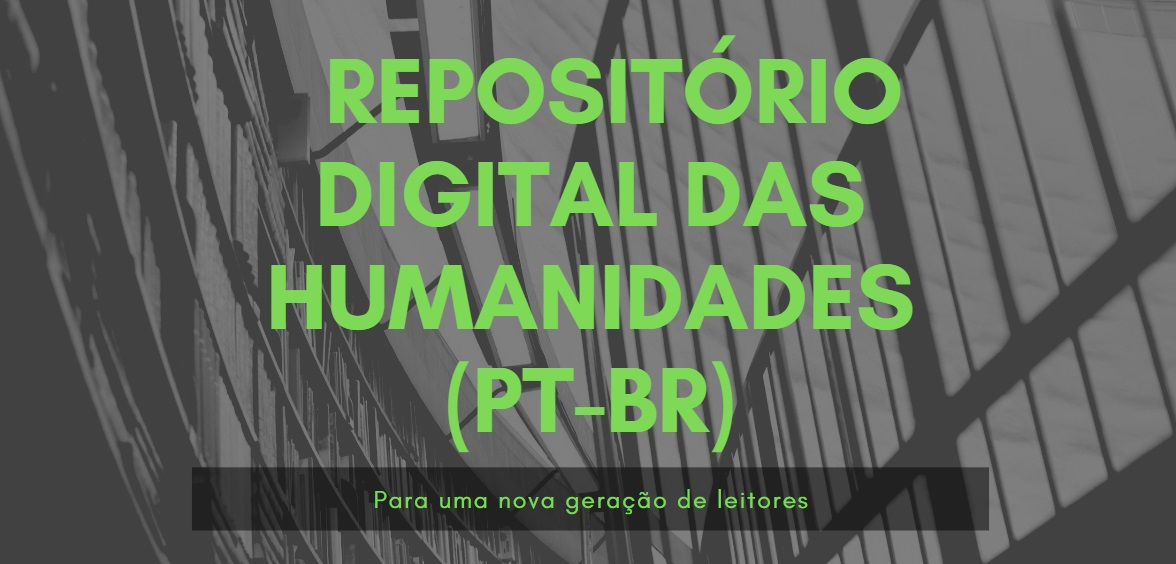
\includegraphics[width=1\textwidth,height=\textheight]{./img/logo.jpg}}
\author{Leonardo F. Nascimento\footnote{UFBA/ICTI/LABHDUFBA/PPGCS, \href{mailto:leofn@ufba.br}{\nolinkurl{leofn@ufba.br}}} \and Eric Brasil\footnote{UNILAB - LABHDUFBA, \href{mailto:profericbrasil@unilab.edu.br}{\nolinkurl{profericbrasil@unilab.edu.br}}} \and Gabriel Andrade\footnote{LABHDUFBA, \href{mailto:gabriel.andrad4@gmail.com}{\nolinkurl{gabriel.andrad4@gmail.com}}} \and Tarssio Barreto\footnote{LABHDUFBA, \href{mailto:tarssioesa@gmail.com}{\nolinkurl{tarssioesa@gmail.com}}} \and Vítor Mussa\footnote{UFRJ/PPGSA/DTA - LABHDUFBA, \href{mailto:vtrmussa@gmail.com}{\nolinkurl{vtrmussa@gmail.com}}} \and Daniel Mendes\footnote{UFRJ/PATHS, \href{mailto:daniel_mnds34@hotmail.com}{\nolinkurl{daniel\_mnds34@hotmail.com}}}}
\date{2021-04-28}

\begin{document}
\maketitle

{
\setcounter{tocdepth}{1}
\tableofcontents
}
\hypertarget{apresentauxe7uxe3o}{%
\chapter{Apresentação}\label{apresentauxe7uxe3o}}

A ideia desta obra foi reunir esforços de diferentes pesquisadores e instituições na elaboração de scripts para coletar - de modo automatizado - a produção intelectual dos principais congressos e eventos das áreas das humanidades.

Além disso, nós tivemos como objetivo mais amplo enfatizar a importância do desenvolvimento de habilidades computacionais por parte dos pesquisadores em todos os campos das humanidades.

Os scripts, as bases de dados e todos os documentos estão disponíveis e poderão ser baixados com apenas um clique. O acervo servirá para a realização de investigações sobre os mais variados aspectos e ampliar, com isso, o conhecimento sobre a produção acadêmica, científica e intelectual do Brasil das ciências humanas e sociais ao longo de décadas.

Para o lancamento, nós escolhemos o \href{https://dhcenternet.org/initiatives/day-of-dh/2021}{Dia Internacional das Humanidades Digitais} em 29/04/2021.

Ao compartilhar nas redes, pedimos que usem a hashtag \textbf{\#dayofdh21}

\begin{figure}
\centering

\includegraphics[width=0.35\textwidth,height=\textheight]{./img/dayofdh.jpg}
\caption{Símbolo do \#dayofdh21}
\end{figure}

\hypertarget{webscraping-e-ciuxeancias-sociais}{%
\chapter{2 Webscraping e ciências sociais}\label{webscraping-e-ciuxeancias-sociais}}

\hypertarget{por-que-automatizar}{%
\section{2.1 Por que automatizar?}\label{por-que-automatizar}}

A dataficação e a digitalização tornaram-se fenomenos massivos das sociedades contemporâneas. Ao interargirmos com as tecnologias digitais nós deixamos traços de dados que podem ser usados para a pesquisa sobre a sociedade. O desafio colocado para os pesquisadores das humanidades está em acessar e manipular tais dados:

\begin{quote}
``Como uma técnica de extração de dados online, o {[}webscraping{]} parece de interesse especial para nós porque é uma parte importante do que torna a pesquisa social digital praticamente possível.'' \href{https://www.tandfonline.com/doi/abs/10.1080/17530350.2013.772070}{(MARRES, N. \& WELTEVREDE, E. Scraping the Social? Journal of Cultural Economy, v. 6, n.~3, p.~313--335, 1 ago. 2013, p.317)}
\end{quote}

O volume, quantidade e qualidade dos dados digitais e digitalizados nunca foi tão grande. O acesso à fontes digitalizadas através de mecanismos de busca por palavras-chave, por assuntos, por metadatos em geral, os milhares de dados produzidos a cada segundo nas redes sociais ou o volume de publicações acadêmicas têm impactado as pesquisas e a própria construção do conhecimento nas ciências humanas e sociais.

Assim, é urgente a necessidade de enfrentarmos os desafios metodológicos e teóricos colocados por esse cenário. A automatização na coleta de dados na Web não é apenas uma forma de acelarar essa relação do pequisador com os dados, mas de qualificar e potencializar a tarefa heurística de seleção dos mesmos.

\hypertarget{como-comeuxe7ar}{%
\section{2.2 Como começar?}\label{como-comeuxe7ar}}

É preciso aprender algum tipo de linguagem de programação (geralmente R ou Python), além de conhecimentos em HTML, CSS e XPATH. Sabemos que, à primeira vista, parecem ser termos complicados para quem vem ``das humanas'', mas o entendimento destas coisas é relativamente mais simples que muitas das leituras que nós fazemos.

Portanto, talvez o primeiro passo seja buscar compreender a estrutura da página que abriga os dados que você pretende coletar. Para isso, é preciso conhecer o mínimo de HTML.

Em seguida é importante definir quais dados e informações você pretende coletar e qual a estrtura de organização você pretende construir como resultado. Esse é um procedimento metodológico fundamental para a pesquisa e demanda do pesquisador o mesmo rigor acadêmico do trabalho com dados de outra natureza.

Por fim, a escrita do código, utilizando a linguagem que melhor atenda aos seus interesses.

Todos esses processos demandam um empenho de tempo e formação técnicas específicas, sem dúvida. Entretanto, acreditamos que os retornos possíveis justificam o investimento de tempo. Além disso, amplia as possibilidades de trabalho interdisciplinar, colaborativo e aberto.

\hypertarget{webscraping-enquanto-tuxe9cnica-das-humanidades}{%
\section{2.3 Webscraping enquanto técnica das humanidades}\label{webscraping-enquanto-tuxe9cnica-das-humanidades}}

Ao realizarmos um webscrapig é preciso atentar para os procedimentos não apenas ``técnicos'' envolvidos na raspagem mas, também, para os aspectos analíticos e epistemológicos. Cada plataforma, website ou \href{https://canaltech.com.br/software/o-que-e-api/}{API} possui características particulares que vão, juntamente com o código que vamos contruir, determinar o tipo e natureza dos dados coletados.

\begin{quote}
A raspagem, entretanto, não é apenas uma técnica, mas também envolve uma forma particular de lidar com a informação e o conhecimento: é também uma prática analítica.\href{https://www.tandfonline.com/doi/abs/10.1080/17530350.2013.772070}{(MARRES, N. \& WELTEVREDE, E. Scraping the Social? Journal of Cultural Economy, v. 6, n.~3, p.~313--335, 1 ago. 2013, p.317)}
\end{quote}

Erros no código de raspagem podem produzir dados distorcidos, com lacunas ou mesmo em duplicidade. Podemos, então, considerar que um erro no código torna-se um erro metodológico.

\hypertarget{linguagens-de-programauxe7uxe3o}{%
\chapter{Linguagens de programação}\label{linguagens-de-programauxe7uxe3o}}

\hypertarget{r}{%
\section{R}\label{r}}

\hypertarget{python}{%
\section{Python}\label{python}}

Alguns dos códigos que compõe o Redhbr foram escritos em \href{https://www.python.org/}{Python 3.8}. Esta é uma linguagem de programação que permite ao programados trabalhar rapidamente e integrar diferentes sistemas com maior eficiência.

\begin{quote}
Foi lançada por Guido van Rossum em 1991. Atualmente, possui um modelo de desenvolvimento comunitário, aberto e gerenciado pela organização sem fins lucrativos \href{https://www.python.org/psf/}{Python Software Foundation}.\footnote{\href{https://pt.wikipedia.org/wiki/Python}{Python - Wikipedia.org}}
\end{quote}

Parte da filosofia da linguagem está resumida no poema \emph{Zen of Python}, \href{https://pt.wikipedia.org/wiki/Python}{escrito por Tim Peters em 1999}.

\begin{quote}
Bonito é melhor que feio
Explícito é melhor que implícito
Simples é melhor que complexo
Complexo é melhor que complicado
Linear é melhor do que aninhado
Esparso é melhor que denso
Legibilidade conta
Casos especiais não são especiais o bastante para quebrar as regras.
Ainda que praticidade vença a pureza
Erros nunca devem passar silenciosamente.
A menos que sejam explicitamente silenciados
Diante da ambiguidade, recuse a tentação de adivinhar
Deveria haver um --- e preferencialmente apenas um --- modo óbvio para fazer algo.
Embora esse modo possa não ser óbvio a princípio a menos que você seja holandês
Agora é melhor que nunca
Embora nunca freqüentemente seja melhor que já
Se a implementação é difícil de explicar, é uma má ideia
Se a implementação é fácil de explicar, pode ser uma boa ideia
Namespaces são uma grande ideia --- vamos ter mais dessas!\footnote{\href{https://pt.wikipedia.org/wiki/Zen_of_Python}{Zen of Python - Wikipedia.org}}
\end{quote}

Para executar um arquivo .py é preciso instalar o Python3 em seu computador.

\href{https://python.org.br/instalacao-windows/}{Clique aqui} para um tutorial de instalação do Python no Windows, \href{https://python.org.br/instalacao-linux/}{clique aqui} para Linux e \href{https://python.org.br/instalacao-mac/}{clique aqui}
para Mac.

Após a instalação, vc pode executar o arquivo .py direto do prompt de comando do Windows ou pelo terminal do Linux, ou utilizar as diversas \href{https://pt.wikipedia.org/wiki/Ambiente_de_desenvolvimento_integrado}{IDE} disponíveis.

Segue um exemplo de como executar utilizando o terminal do Linux, após instalar o Python3.8:

\begin{enumerate}
\def\labelenumi{\arabic{enumi}.}
\tightlist
\item
  Acesse o diretório em que o arquivo .py está salvo:
\end{enumerate}

sh
\texttt{\$\ cd\ "caminho\ do\ diretório"}

\begin{enumerate}
\def\labelenumi{\arabic{enumi}.}
\tightlist
\item
  Instale as bibliotecas requeridas:
\end{enumerate}

sh
\texttt{\$\ pip3\ install\ -r\ requirements.txt}

\begin{enumerate}
\def\labelenumi{\arabic{enumi}.}
\tightlist
\item
  Execute o arquivo usando Python3.8
\end{enumerate}

sh
\texttt{\$\ python3\ script-anais-anpuh.py}

\hypertarget{anpuh}{%
\chapter{ANPUH}\label{anpuh}}

\hypertarget{o-que-uxe9-anpuh}{%
\section{O que é ANPUH?}\label{o-que-uxe9-anpuh}}

A \href{https://anpuh.org.br/index.php}{Associação Nacional de História, Anpuh}, fundada em 1961, inicialmente destinada aos docentes de cursos de graduação e pós-graduação. Em 1993, a ANPUH ampliou sua base para todoa os profissionais de história.

\begin{quote}
A cada dois anos, a ANPUH realiza o Simpósio Nacional de História, o maior e mais importante evento da área de história no país e na América Latina\footnote{\href{https://anpuh.org.br/index.php/quem-somos}{Anpuh-Quem somos}}.
\end{quote}

Desenvolvemos scripts diferentes para dois tipos de conjuntos de dados relacionados à Associação Nacional de História.

\begin{itemize}
\item
  Anais-Anpuh: script para raspagem de todos os trabalhos publicados nos Anais dos Simpósio Nacionais de História entre 1963 e 2017, disponíveis no site da Anpuh.
\item
  anpuh-scraper: script para raspagem dos resumos (e demais informações) de todos os trabalhos aprovados para todos os simpósios temáticos dos SNH nos aos de 2013, 2015, 2017 e 2019.
\end{itemize}

\hypertarget{scripts-de-raspagem}{%
\section{Scripts de raspagem}\label{scripts-de-raspagem}}

\hypertarget{anais-em-pdf-da-anpuh}{%
\subsection{Anais em pdf da ANPUH}\label{anais-em-pdf-da-anpuh}}

\href{https://github.com/LABHDUFBA/Anais-Anpuh}{\textbf{Clique aqui para acessar o repositório no Github}}

Esse script realiza a raspagem dos trabalhos em PDF de todos os Simpósios Nacionais da Anpuh entre 1963 até 2017, disponíveis atualmente na site da associação, que podem ser \href{https://anpuh.org.br/index.php/documentos/anais}{acessados aqui}.

Escrito em \href{https://www.python.org/}{Python 3.8}, o script utiliza as seguintes bibliotecas e módulos

\begin{itemize}
\tightlist
\item
  \textbf{urllib.requests}: módulo do Python para acessar urls. \href{https://docs.python.org/pt-br/3/library/urllib.request.htmll}{Saiba mais.}
\item
  \textbf{os}: módulo do Python que permite manipular funções do sistema operacional. \href{https://docs.python.org/pt-br/3/library/os.html}{Saiba mais.}
\item
  \textbf{bs4}: \href{https://www.crummy.com/software/BeautifulSoup/bs4/doc/}{Beautiful Soup} é uma biblioteca Python para extrair dados de arquivos HTML e XML.
\item
  \textbf{re}: \href{https://docs.python.org/pt-br/3/library/re.html}{Regular Expressions} é um módulo do Python para operar com expressões regulares.
\item
  \textbf{pandas}: \href{https://pandas.pydata.org/}{Pandas} é uma biblioteca escrita em Python para manipulação e análise de dados.
\item
  \textbf{wget}: \href{https://pypi.org/project/wget/}{Wget} é uma biblioteca escrita em Python para realizar downloads.
\end{itemize}

O script tem o seguinte funcionamento quando executado:

\begin{itemize}
\tightlist
\item
  Cria pasta para salvar os PDFs, após verificar se a mesma não existe no local: \texttt{Anais\ Anpuh\textgreater{}\ pdf} utilizando módulo \texttt{os}.
\item
  Acessa a URL dos Anais com a biblioteca \texttt{urllib} e realiza a análise do HTML da mesma com a biblioteca \texttt{BeautifulSoup};
\item
  Cria uma lista de eventos a partir da página principal;
\item
  Acessa as páginas de cada evento contidas na lista criada anteriormente através de uma iteração;
\item
  Em cada item da lista de eventos, o script busca todos os papers da primeira página e cria uma nova lista. Nessa lista de papers de uma dada página o script realizará as seguintes ações:

  \begin{itemize}
  \tightlist
  \item
    encontrar as informações de cada paper;
  \item
    inclui essas informações em uma lista (que depois gerará um CSV com os dados);
  \item
    busca se há pdf disponível e se ele não é repetido faz download do PDF
  \item
    Após realizar essas ações para todos os itens de uma página, busca a próxima página de papers do evento, se não houver, passa para o próximo evento e repete as ações em um \emph{loop} até o último evento disponível.
  \end{itemize}
\end{itemize}

\hypertarget{dados}{%
\subsection{Dados}\label{dados}}

O script retorna para o usuário \textbf{todos os pdfs disponíveis em todas as páginas de todos os Simpósios Nacionais da Anpuh desde 1963 até 2017}. São criadas pastas com o número de cada evento para o armazenamento dos arquivos em PDF.

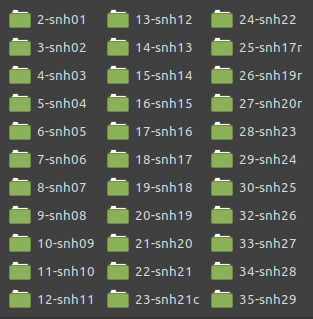
\includegraphics{img/pastas.png}

É importante notar que muitos papers não estão com pdf disponível no site, assim como nas edições mais antigas encontramos arquivos que contém vários papers num único PDF.

O script também gera um arquivo \textbf{CSV} (\emph{comma-separated values}) contendo os seguintes valores para cada paper: Autor(es)/Instituições,Título, Tipo, Evento, Ano, Link do Arquivo. Esse arquivo pode ser aberto como uma planilha e trabalhado em banco de dados.

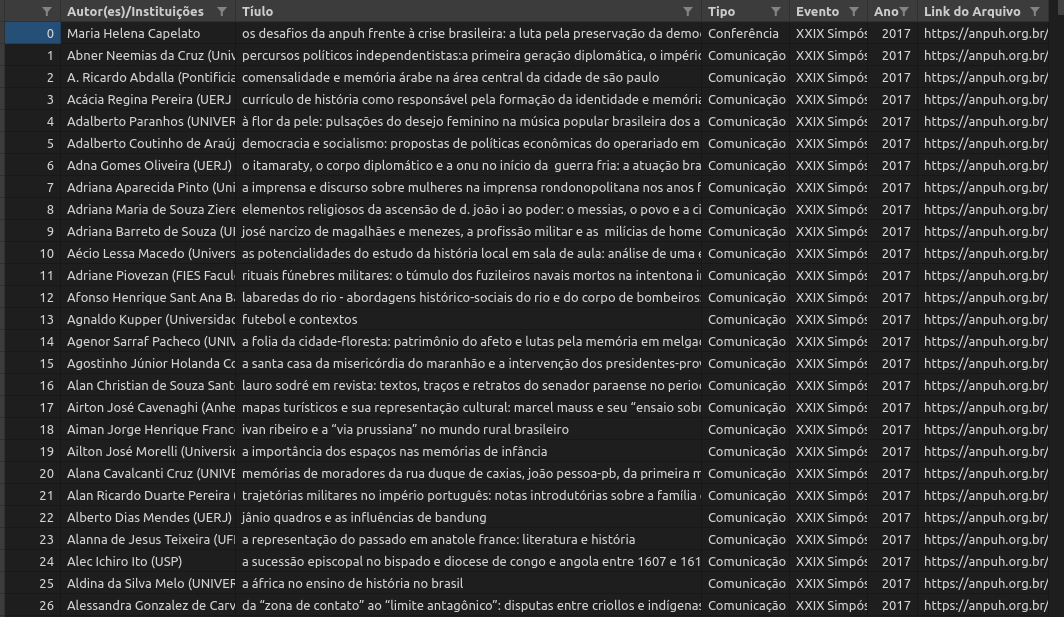
\includegraphics{img/ex_csv1.png}

\hypertarget{resumos-dos-trabalhos-da-anpuh}{%
\subsection{Resumos dos trabalhos da ANPUH}\label{resumos-dos-trabalhos-da-anpuh}}

\href{https://github.com/LABHDUFBA/anpuh-scraper}{\textbf{Clique aqui para acessar o repositório no Github}}.

\emph{Raspador dos resumos dos Simpósios Nacionais de História da \href{https://anpuh.org.br}{Associação Nacional de História - Anpuh}. O programa raspa todos os resumos dos SNH 27, 28, 29 e 30, respectivamente dos anos de 2013, 2015, 2017 e 2019}
Escrito em \href{https://www.python.org/}{Python 3.8}, o script utiliza as seguintes bibliotecas e módulos

\begin{itemize}
\tightlist
\item
  \textbf{urllib.requests}: módulo do Python que ajuda a acessar urls.
  \href{https://docs.python.org/pt-br/3/library/urllib.request.htmll}{Saiba mais.}
\item
  \textbf{bs4}: \href{https://www.crummy.com/software/BeautifulSoup/bs4/doc/}{Beautiful Soup} é uma biblioteca Python para extrair dados de arquivos HTML e XML.
\item
  \textbf{pandas}: \href{https://pandas.pydata.org/}{Pandas} é uma biblioteca escrita em Python para manipulação e análise de dados.
\end{itemize}

O script tem o seguinte funcionamento quando executado:

Pergunta ao usuário que ano pretende raspar e se deseja incluir um novo ano à lista.
Após a criação da lista com os anos escolhidos pelo usuário, o script acessa cada uma das páginas com as listas dos STs nos sites de cada evento;
Acessa cada ST, encontra os dados de todos os resumos e passa para o ST seguinte;
Após terminar um ST, passa para o próximo evento e executa as mesmas função;
Todos os dados são inseridos em um DataFrame em Pandas e ao final são salvos no formato CSV.

\hypertarget{dados-1}{%
\subsection{Dados}\label{dados-1}}

O script retorna para o usuário um \textbf{CSV (\emph{comma-separated values}) com os dados de todos os trabalhos aceitos nos Simpósio Temáticos dos SNH 27, 28, 29 e 30}.

O CSV contém as seguintes variáveis para cada resumo:

\texttt{Ano,\ Evento,\ Cidade,\ ST,\ Coordenadores,\ Autor(es)/Instituições,\ Título,\ Resumo}

Esse arquivo pode ser aberto como uma planilha e trabalhado em banco de dados.

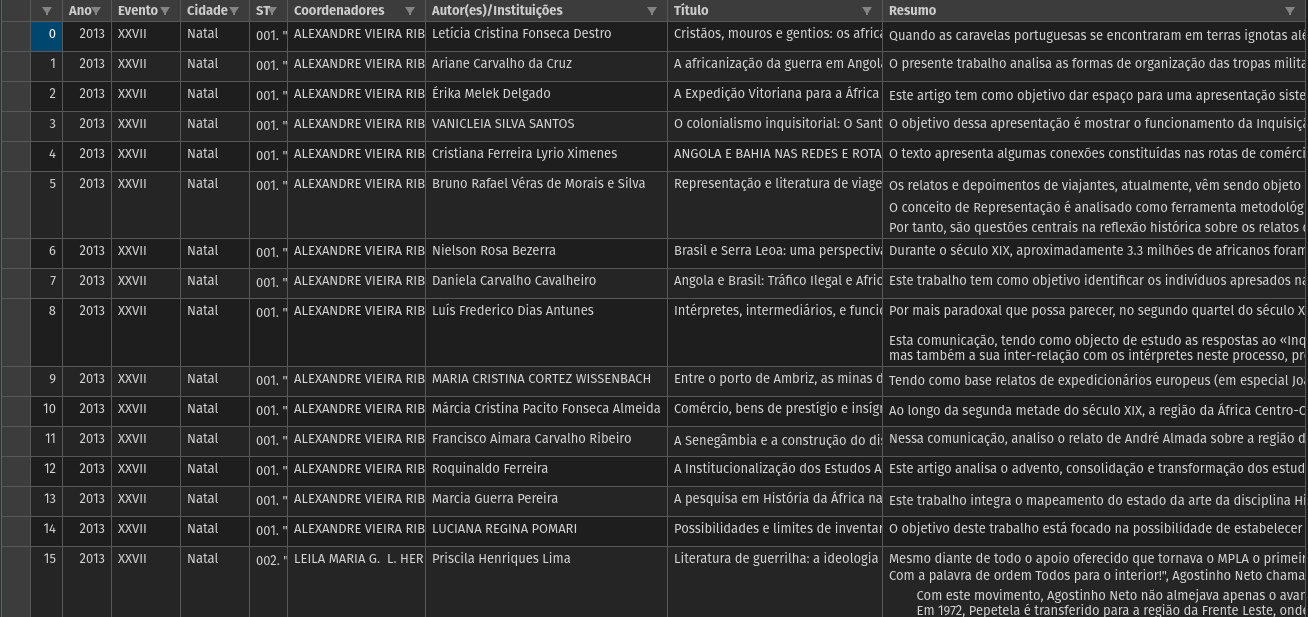
\includegraphics{img/ex_csv2.png}

\hypertarget{anpocs}{%
\chapter{ANPOCS}\label{anpocs}}

\hypertarget{o-que-uxe9-a-anpocs}{%
\section{O que é a ANPOCS?}\label{o-que-uxe9-a-anpocs}}

A \href{http://anpocs.com/}{Associação Nacional de Pós-Graduação e Pesquisa em Ciências Sociais (ANPOCS)} é uma entidade de direito privado sem fins lucrativos que reúne centenas de centros de pós-graduação e de pesquisa em antropologia, ciência política, relações internacionais e sociologia de todo o Brasil. Ela é formada, portanto, por instituições, em vez de pesquisadores individuais.

A associação organiza os \emph{Encontros Anuais da ANPOCS}, que consistem em congressos cujo número médio de participantes é de 1500 pesquisadores. Esses encontros estão entre os fóruns mais relevantes para as ciências sociais no Brasil.

Diante disso, desenvolvemos o \texttt{anpocs-scraper} -- \href{https://github.com/vmussa/anpocs-scraper}{disponível aqui} --, um raspador que permite coletar de forma automatizada os dados dos resumos dos trabalhos apresentados nos encontros de 2019, 2020 e, futuramente, 2021. O raspador expressa mais uma iniciativa que busca contribuir para uma ciência aberta e transparente, facilitando o acesso aos dados dos congressos e contribuindo para a preservação da memória das ciências sociais brasileiras.

\hypertarget{script-de-raspagem}{%
\section{Script de raspagem}\label{script-de-raspagem}}

\hypertarget{anpocs-scraper}{%
\subsection{anpocs-scraper}\label{anpocs-scraper}}

\includegraphics{img/demo.gif}

O \texttt{anpocs-scraper} é um raspador dos dados dos \href{http://anpocs.com/index.php/encontros/apresentacao}{Encontros Anuais da ANPOCS} escrito em Python. Atualmente o código permite coletar:

\begin{itemize}
\item
  os dados de todos os resumos dos trabalhos apresentados em GT's e SPG's do \href{https://www.anpocs2020.sinteseeventos.com.br/}{44º Encontro Anual da ANPOCS}
\item
  os dados de todos os resumos dos trabalhos apresentados em ST's e SPG's do \href{http://anpocs.com/index.php/43-encontro-anual-2019/2750-encontros-anuais/43-encontro/2301-resumos-sts-e-spgs}{43º Encontro Anual da ANPOCS}
\end{itemize}

\hypertarget{instalauxe7uxe3o-e-modo-de-uso}{%
\subsection{Instalação e modo de uso}\label{instalauxe7uxe3o-e-modo-de-uso}}

Para instalar o raspador basta clonar o repositório, \href{https://github.com/vmussa/anpocs-scraper}{que se encontra aqui}, e instalar suas dependências:

\begin{verbatim}
git clone https://github.com/vmussa/anpocs-scraper
cd anpocs-scraper
python -m venv .venv && source .venv/bin/activate
pip install -r requirements.txt
\end{verbatim}

Para rodar o raspador, continue no repositório clonado e execute o código \texttt{main.py} com o Python:

\begin{verbatim}
python src/main.py
\end{verbatim}

\begin{quote}
Atenção → \textbf{para realizar esse procedimento, você precisa instalar o Google Chrome e o ChromeDriver}: \href{https://chromedriver.chromium.org/getting-started}{Clique aqui} para ler um tutorial sobre como instalar o ChromeDriver.
\end{quote}

\hypertarget{dados-2}{%
\section{Dados}\label{dados-2}}

O programa exporta, para cada edição do congresso, uma tabela no formato CSV com as seguintes informações de cada trabalho apresentado:

\begin{quote}
\texttt{autores}, \texttt{titulo}, \texttt{resumo}, \texttt{sessao}, \texttt{id\_evento}
\end{quote}

A imagem abaixo ilustra o formato de uma das tabelas:

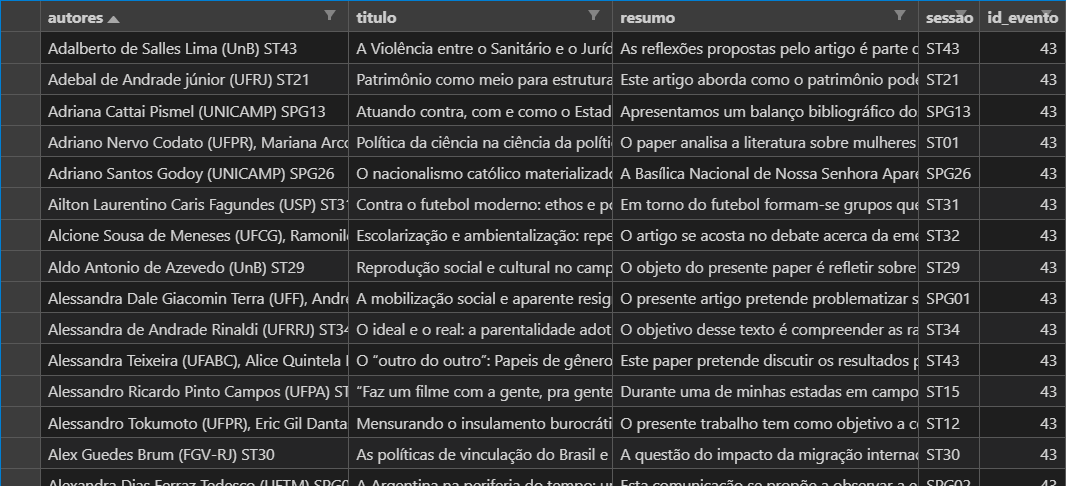
\includegraphics{img/anpocs_scraper_csv.png}

Caso você não queira rodar o raspador, mas precise dos dados, você pode obter \href{https://drive.google.com/drive/folders/1XdHLf3b7r0d1EwwlYo4D0bRBujVILBq7?usp=sharing}{a versão atual do conjunto de dados exportado pelo programa aqui}.

\hypertarget{em-breve}{%
\section{Em breve}\label{em-breve}}

Futuramente o raspador abarcará todos os GT's e SPG's do encontro 45, cujos resumos dos trabalhos estarão disponíveis aqui. Além disso, ele contará com um módulo de limpeza dos dados que fará o pré-processamento para a análise qualitativa e/ou computacional. Por fim, disponibilizaremos, também, todos os PDFs de artigos enviados para todas as edições dos Encontros Anuais da ANPOCS.

\hypertarget{compuxf3s}{%
\chapter{COMPÓS}\label{compuxf3s}}

\hypertarget{o-que-uxe9-a-compuxf3s}{%
\section{O que é a COMPÓS?}\label{o-que-uxe9-a-compuxf3s}}

\href{https://www.compos.org.br/a_compos.php}{A COMPÓS - Associação Nacional dos Programas de Pós-Graduação em Comunicação - foi fundada em 16 junho de 1991, em Belo Horizonte, com o apoio da Capes e do CNPq, a partir da iniciativa de alguns pesquisadores e representantes dos seguintes cursos de Pós-Graduação: PUC-SP, UFBA, UFRJ, UnB, UNICAMP, UMESP. É uma sociedade civil, sem fins lucrativos, congregando como associados os Programas de Pós-Graduação em Comunicação em nível de Mestrado e/ou Doutorado de instituições de ensino superior públicas e privadas no Brasil. A COMPÓS tem como objetivos principais o fortalecimento e qualificação crescentes da Pós-Graduação em Comunicação no país; a integração e intercâmbio entre os Programas existentes, bem como o apoio à implantação de novos Programas; o diálogo com instituições afins nacionais e internacionais; o estímulo à participação da comunidade acadêmica em Comunicação nas políticas do país para a área, defendendo o aperfeiçoamento profissional e o desenvolvimento teórico, cultural, científico e tecnológico no campo da Comunicação.}

\href{https://www.compos.org.br/encontros_anuais.php}{Como espaço de intercâmbio acadêmico entre os pesquisadores dos vários Programas, a COMPÓS tem como fórum privilegiado os Encontros Anuais, estruturados sob a forma de Grupos de Trabalhos (GTs), onde são apresentados e debatidos estudos que buscam refletir sobre o avanço científico, tecnológico e cultural no campo da comunicação}

Diante disso, desenvolvemos o \texttt{Anais-COMPOS-scraper} -- \href{https://github.com/LABHDUFBA/Anais-COMPOS-scraper}{disponível aqui} -- que realiza o download automatizado de todos os papers em pdf dos Encontros da COMPÓS entre 2000 até 2020 (disponíveis atualmente na site). Além disso, o script também gera um arquivo CSV (comma-separated values) contendo as seguintes informações para cada paper: Ano, Edição, Nome do GT, Título, Autores, e Link do Arquivo. Esse arquivo pode ser aberto como uma planilha e trabalhado em banco de dados.

O raspador expressa mais uma iniciativa que busca contribuir para uma ciência aberta e transparente, facilitando o acesso aos dados dos congressos e contribuindo para a preservação da memória das ciências sociais brasileiras.

\hypertarget{script-de-raspagem-1}{%
\section{Script de raspagem}\label{script-de-raspagem-1}}

\hypertarget{r-e-rstudio}{%
\subsection{R e RStudio}\label{r-e-rstudio}}

O R e RStudio são gratuitos e possuem versões para Windows, Mac e Linux. A instalação é bastante fácil e em geral você apenas tem que seguir as instruções da tela.

Para instalar o R, baixe a versão adequada para seu computador em: \url{https://cloud.r-project.org/}

Para instalar o RStudio, baixe a versão adequada para seu computador em: \url{https://www.rstudio.com/products/rstudio/download/}

Além disso, para ter um ambiente completo de desenvolvimento no R, recomendamos, adicionalmente, instalar:

-- MikTex (para Windows: \url{http://miktex.org/download} ou MacTex (para Mac: \url{https://tug.org/mactex/downloading.html} para relatórios em latex.

-- RTools (para Windows: \url{https://cran.r-project.org/bin/windows/Rtools/} ou Xcode com command line tools (para Mac na AppStore do Mac), para criar pacotes, usar C++ com R entre outras coisas

Após a instalação, vc pode executar o arquivo \textbf{compos.R} que está na pasta \textbf{R} direto do RStudio.

\hypertarget{bibliotecas-e-muxf3dulos}{%
\subsection{Bibliotecas e módulos}\label{bibliotecas-e-muxf3dulos}}

Vocêr vai precisar instalar as seguintes bibliotecas:

\begin{enumerate}
\def\labelenumi{\arabic{enumi}.}
\tightlist
\item
  \href{https://cran.r-project.org/web/packages/RSelenium/RSelenium.pdf}{RSelenium}
\item
  \href{https://www.tidyverse.org/}{tidyverse}
\item
  \href{https://cran.r-project.org/web/packages/rvest/rvest.pdf}{rvest}
\end{enumerate}

\hypertarget{chromedriver}{%
\subsection{Chromedriver}\label{chromedriver}}

\begin{enumerate}
\def\labelenumi{\arabic{enumi}.}
\item
  \href{https://www.youtube.com/watch?v=dz59GsdvUF8}{Instruções sobre como instalar o Chromedriver no Windows 10 :}
\item
  \href{https://medium.com/@marco.conviccao/configurando-o-chromedriver-no-ubuntu-7baaf2be7c68}{Instruções sobre como instalar o Chromedriver no Ubuntu :}
\end{enumerate}

\hypertarget{dados-3}{%
\section{Dados}\label{dados-3}}

O programa exporta, para cada edição do congresso, uma tabela no formato CSV com as seguintes informações de cada trabalho apresentado:

\begin{quote}
\texttt{Ano}, \texttt{Edição}, \texttt{Nome\ do\ GT}, \texttt{Título}, \texttt{Autores}, \texttt{Links}.
\end{quote}

A imagem abaixo ilustra o formato de uma das tabelas:

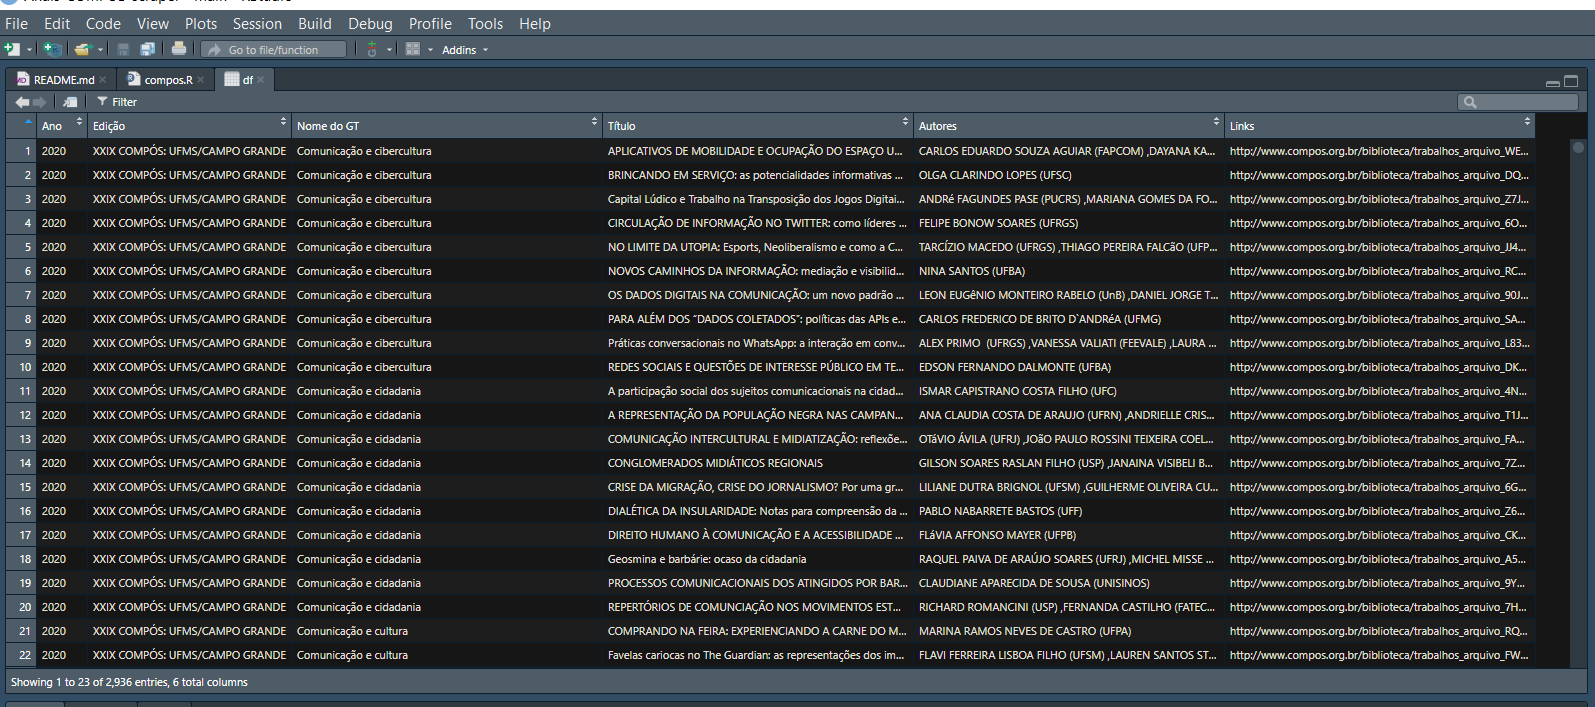
\includegraphics{img/csv.png}

\href{https://filesender.rnp.br/?s=download\&token=ae3e90f6-c8db-497f-a3e0-73958c634997}{Se preferir baixar a base dos PDFs sem usar o código clique aqui.}
(\textbf{OBS:a nomeação ainda contém alguns pequenos erros que serão corrigidos em breve})

\href{https://docs.google.com/spreadsheets/d/1VXlCD9rak-ut3_5p6UFyzOfuSgpbBcl9KDHrXe53q-0/edit?usp=sharing}{Se preferir baixar a planilha sem usar o código clique aqui.}

\hypertarget{sobre-os-autores}{%
\chapter{Sobre os autores}\label{sobre-os-autores}}

\hypertarget{leonardo-f.-nascimento}{%
\section{Leonardo F. Nascimento}\label{leonardo-f.-nascimento}}

Sou formado em Química pelo Instituto Federal de Educação, Ciência e Tecnologia da Bahia -- IFBA (1997), graduado em Psicologia pela Universidade Federal da Bahia -- UFBA (2002), mestre em Sociologia pela Universidade de São Paulo -- USP (2007) e doutor em Sociologia pelo Instituto de Estudos Sociais e Políticos -- IESP/UERJ (2013). Entre 2010 e 2011, realizei estágio doutoral na \emph{École des Hautes Études en Sciences Sociales} (EHESS).

Nos últimos anos estou totalmente dedicado ao estudo das novas tecnologias aplicadas à pesquisa e análise de dados em Ciências Sociais, especialmente com uso de CAQDAS (Computer Assisted/Aided Qualitative Data Analysis). Eu sou professor do Bacharelado Interdisciplinar (BI) em Ciência, Tecnologia e Inovação da UFBA e membro permanente do Programa de Pós-Graduação em Ciências Sociais da UFBA (PPGCS/UFBA). Eu desenvolvo pesquisas sobre sociologia digital, mineração de dados, ciência social computacional e análise de mídia. Em 2018 eu ajudei a criar o Laboratório de Humanidades Digitais da UFBA, uma convergência de pesquisadores e interesses de pesquisa em torno dos temas da ciência social computacional,
humanidades e métodos digitais.

Currículos e redes acadêmicas

\href{https://leofn.com/}{Webpage} -
\href{http://lattes.cnpq.br/7141811368487014}{Lattes} - \href{https://www.linkedin.com/in/leonardo-nascimento-labhdufba/}{LinkedIn} - \href{https://twitter.com/leofn3}{Twitter} -
\href{https://orcid.org/0000-0003-2929-1115}{Orcid} - \href{https://www.researchgate.net/profile/Leonardo-Nascimento-2}{ResearchGate}

\hypertarget{eric-brasil-ihlmunilab}{%
\section{Eric Brasil (IHLM/UNILAB)}\label{eric-brasil-ihlmunilab}}

Professor do curso de licenciatura em História e professor do Bacharelado Interdisciplinar em Humanidades no Instituto de Humanidades e Letras da Universidade da Integração Internacional da Lusofonia Afro-brasileira (IHL-UNILAB), campus dos Malês, Bahia. Doutor (2016) e Mestre (2011) pelo Programa de Pós-Graduação em História Social da Universidade Federal Fluminense. Autor do livro A Corte em Festa: experiências negras em carnavais do Rio de Janeiro (1879-1888) (Editora Prismas, 2016). Vencedor do primeiro lugar no Concurso de Monografias Silvio Romero de 2011 e do segundo lugar em 2020, promovido pelo Centro Nacional de Folclore e Cultura Popular.Foi professor de ensino fundamental, médio e pré-vestibular no Rio de Janeiro entre 2007 e 2017.

Pesquisador do Laboratório de Humanidades Digitais da UFBA. Membro do GT Nacional Emancipações e Pós-Abolição da Anpuh. Tem experiência na área de História Social da Cultura, Humanidades e História Digital, Abolição da escravidão e o Pós-Abolição no Brasil e no Caribe, atuando principalmente nos seguintes temas: Carnaval, Cidadania, História Transnacional, Diáspora Africana, História das Afro-Américas, Hemerotecas e arquivos digitais, métodos digitais de pesquisa, linguagem de programação para a pesquisa em História, web scraping.

Currículos e redes acadêmicas

\href{https://ericbrasiln.github.io}{Webpage} - \href{http://lattes.cnpq.br/6853705640900524}{Lattes} - \href{\%22https://orcid.org/0000-0001-5067-8475}{Orcid} - \href{https://www.researchgate.net/profile/Eric_Brasil}{ResearchGate} - \href{https://unilab.academia.edu/EricBrasil}{Academia.edu}

\hypertarget{vuxedtor-mussa-dtappgsaufrj-e-labhdufbaufba}{%
\section{Vítor Mussa (DTA/PPGSA/UFRJ e LABHDUFBA/UFBA)}\label{vuxedtor-mussa-dtappgsaufrj-e-labhdufbaufba}}

Mestrando do Programa de Pós-Graduação em Sociologia e Antropologia (PPGSA) da Universidade Federal do Rio de Janeiro (UFRJ).

É membro do grupo de pesquisa Desenvolvimento, Trabalho e Ambiente (\href{https://www.nucleodta.org/inicio}{DTA-UFRJ}) e do Laboratório de Humanidades Digitais da Universidade Federal da Bahia (\href{http://www.labhd.ufba.br/}{LABHD-UFBA}).

Currículos e redes acadêmicas

\href{https://vmussa.github.io}{Webpage} - \href{http://lattes.cnpq.br/2934187748254130}{Lattes} - \href{https://www.researchgate.net/profile/Vitor-Mussa-2}{ResearchGate} - \href{https://www.linkedin.com/in/vmussa/}{LinkedIn} - \href{https://twitter.com/vitormussa}{Twitter}

\hypertarget{tarssio-barreto-labhdufba}{%
\section{Tarssio Barreto (LABHDUFBA)}\label{tarssio-barreto-labhdufba}}

Co-fundador da Bit Analytics, doutorando do Programa de Pós Graduação em Engenharia Industrial(PEI/UFBA) com foco na área de técnicas de agrupamentos voltadas para Machine Learning. Mestre em Meio Ambiente Águas e Saneamento - UFBA (2018) e graduado em Engenharia Sanitária e Ambiental pela UFBA (2015). Área de atuação: Machine Learning; modelagem probabilística e simulação e programação avançada em R.\#RStats

\href{http://lattes.cnpq.br/8314700954142455}{Lattes} -
\href{https://www.linkedin.com/in/tarssio-brito-barreto-9646b817b/}{LinkedIn} -
\href{https://twitter.com/danielmnds34}{Twitter}

\hypertarget{daniel-mendes-pathsufrj}{%
\section{Daniel Mendes (PATHS/UFRJ)}\label{daniel-mendes-pathsufrj}}

Graduando no curso de Bacharelado em Ciências Sociais do Instituto de Filosofia e Ciências Sociais (IFCS) da Universidade Federal do Rio de Janeiro (UFRJ).

É membro do grupo de pesquisa Núcleo de Pesquisa em Estratificação e Trajetórias Sociais (\href{https://www.facebook.com/paths.research/}{PATHS}).

Currículos e redes acadêmicas

\href{http://lattes.cnpq.br/9834413442426550}{Lattes} - \href{https://www.linkedin.com/in/daniel-mendes-251212176/}{LinkedIn} - \href{https://twitter.com/danielmnds34}{Twitter}

\hypertarget{gabriel-andrade-labhdufbaufba}{%
\section{Gabriel Andrade (LABHDUFBA/UFBA)}\label{gabriel-andrade-labhdufbaufba}}

Graduando no curso de Bacharelado em Engenharia de Computação da Escola Politécnica da Universidade Federal da Bahia (UFBA)

É desenvolvedor de software e membro do Laboratório de Humanidades Digitais da Universidade Federal da Bahia (\href{http://www.labhd.ufba.br/}{LABHDUFBA}).

Currículos e redes acadêmicas

\href{https://gabrielsandrade.github.io}{Webpage} - \href{http://lattes.cnpq.br/4915378425369073}{Lattes} - \href{https://www.linkedin.com/in/gabriel-andrade-633996108}{LinkedIn} - \href{https://twitter.com/ga_brieell_}{Twitter}

\hypertarget{ajude-o-projeto}{%
\section{Ajude o projeto!}\label{ajude-o-projeto}}

\begin{figure}
\centering

\includegraphics[width=0.35\textwidth,height=\textheight]{C:/Users/Leonardo/Desktop/redhbr/img/btc.png}
\caption{bc1qmug7kcrw3kxklca7chy7c344d62gtc8fhqwnkw}
\end{figure}

  \bibliography{book.bib,packages.bib}

\end{document}
